\chapter{Továbbfejlesztési lehetőségek}\label{ch:továbbfejlesztési-lehetőségek}

A jelenlegi algoritmus legszembetűnőbb hiánya az, hogy csupán két fél tud egymással kommunikálni.
Alapvetően ahhoz, hogy egy csomópont kommunikálni tudjon egy másikkal, az szükséges, hogy ismerjék egymás kulcspárának
publikus részét.
Ezt jelenleg kézzel kell konfigurálni.
A konfigurálandó kulcsok száma a választott hálózati topológiától függ.
Értelemszerűen ez a szám a \emph{full mesh} topológia esetében lesz a legnagyobb, és több ezer csomópont esetén nem fenntartható
az, hogy manuálisan legyen szükséges konfigurálni a kulcsokat minden csomóponton.
Célszerű lehet az algoritmus oly módon módosítani, hogy minimális konfigurációval létre lehessen hozni egy full mesh
hálózatot.

\begin{figure}[!ht]
    \centering
    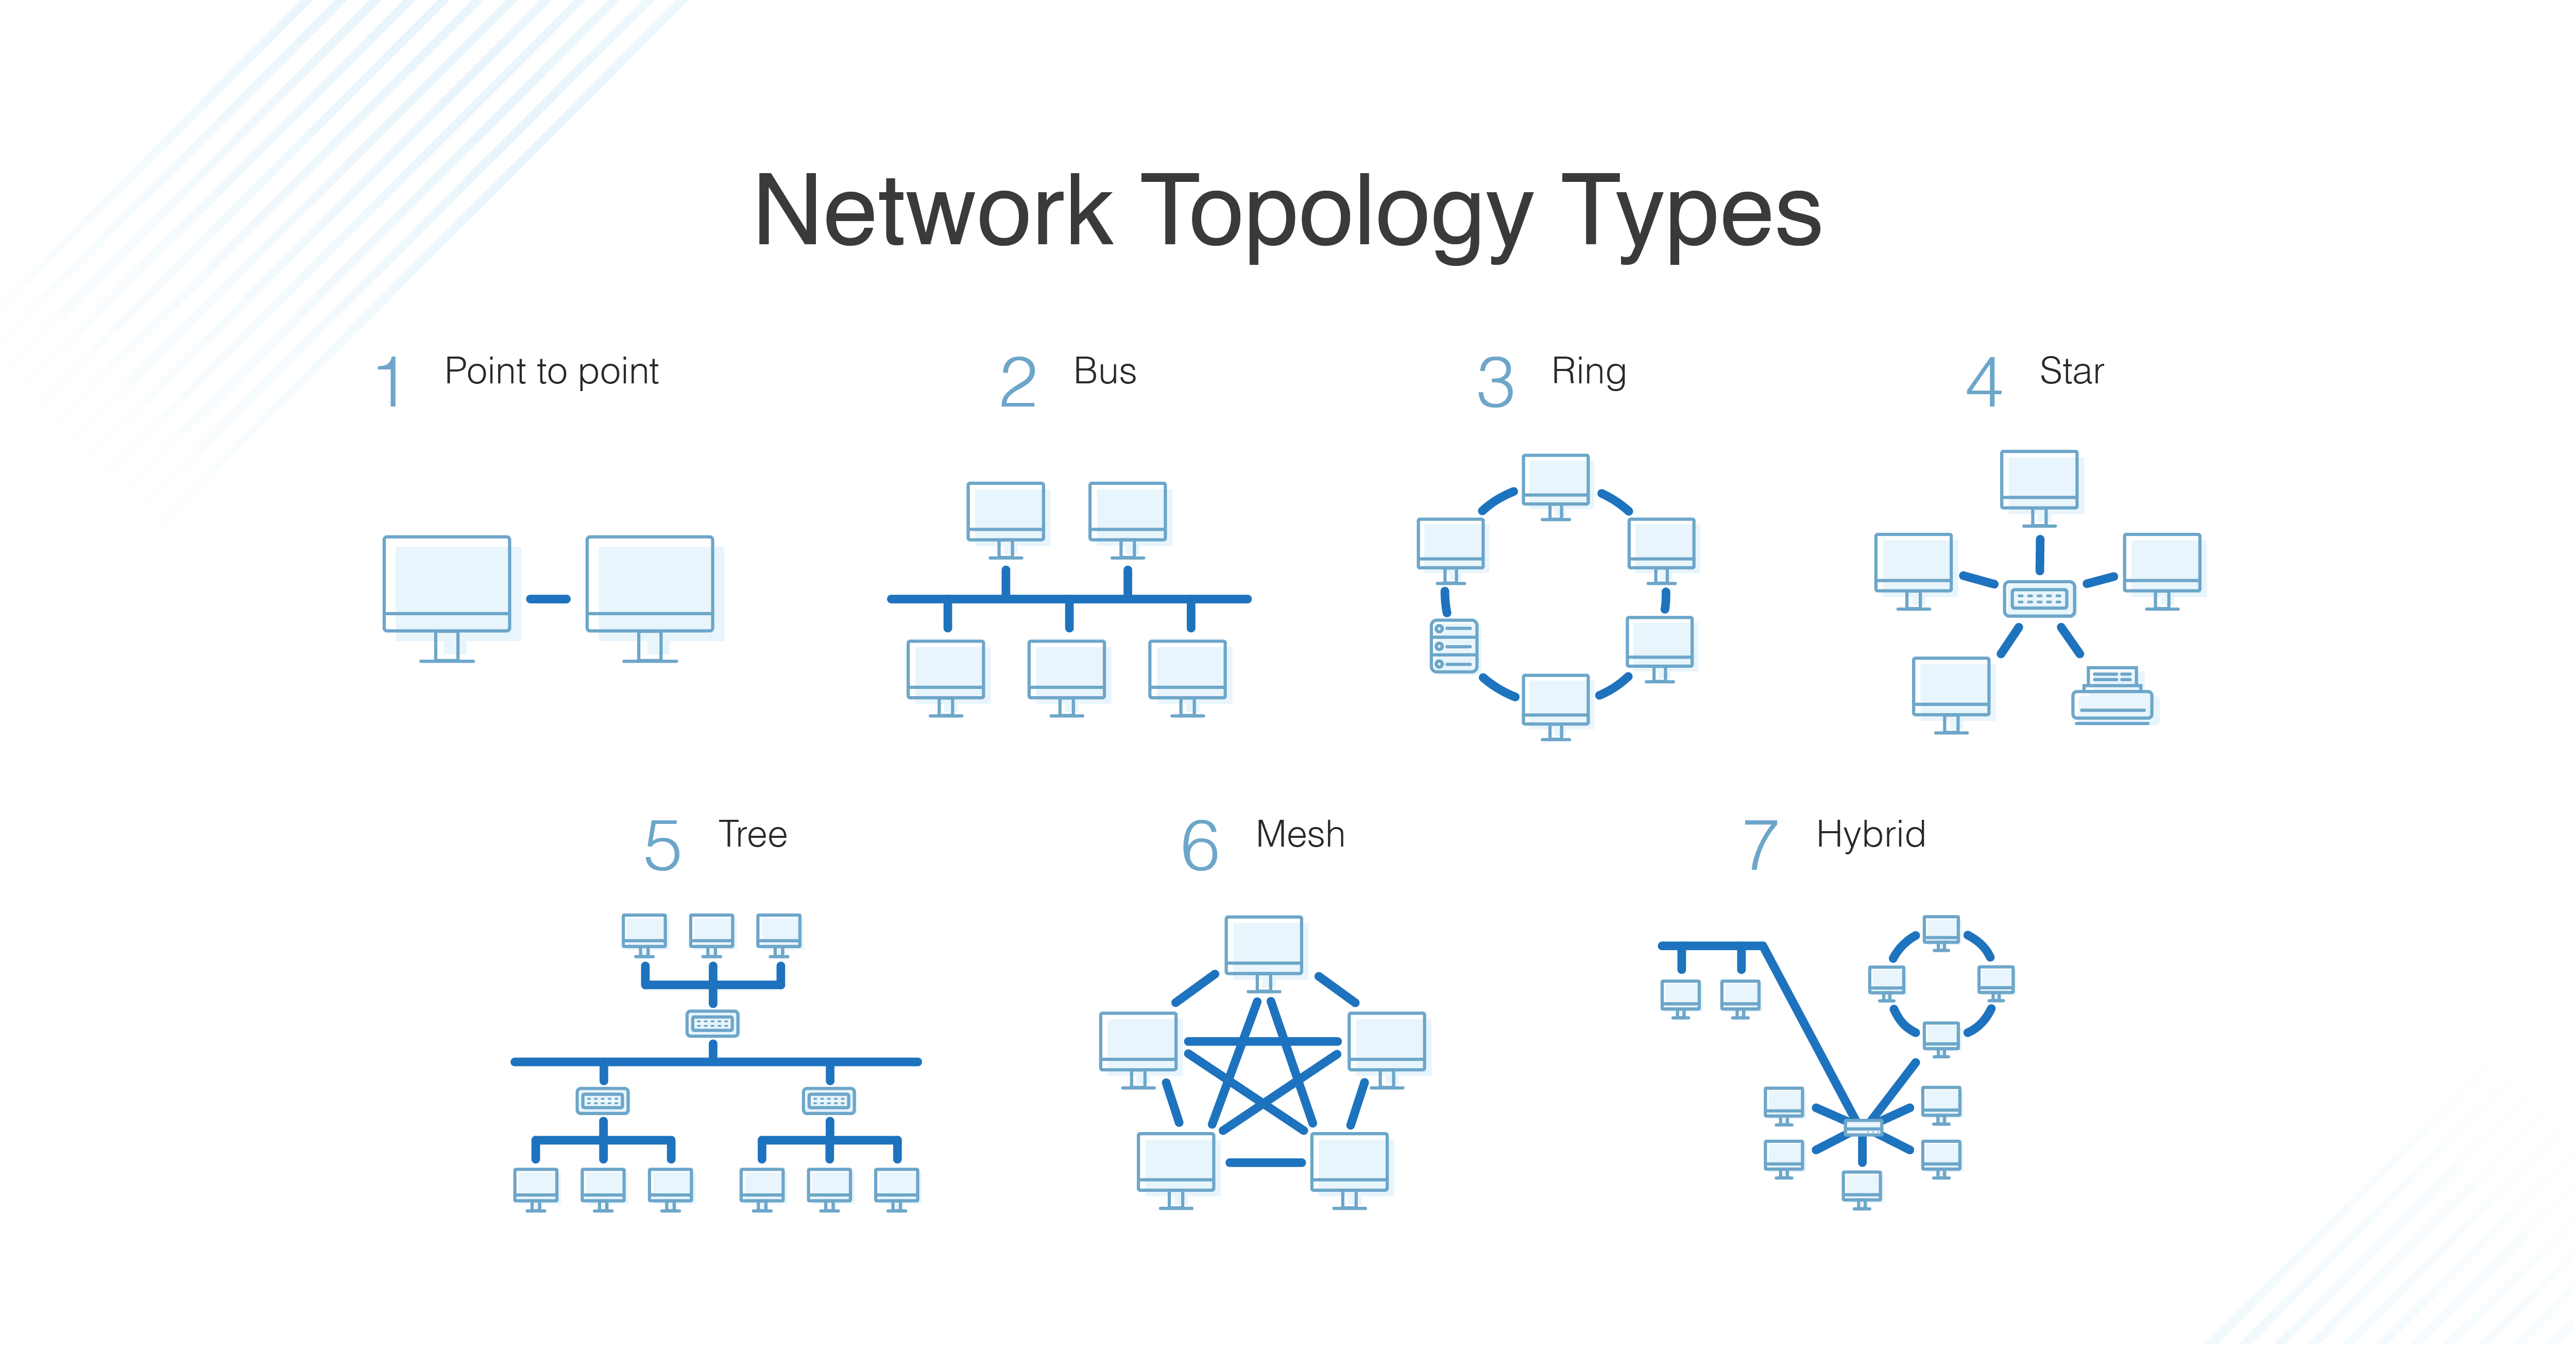
\includegraphics[width=140mm, keepaspectratio]{figures/topology}
    \caption{Különböző hálózati topológiák ábrázolva (forrás: https://www.dnsstuff.com/what-is-network-topology).}
    \label{fig:topo}
\end{figure}

Emellett ahhoz, egy csomópont több másikhoz tudjon csatlakozni, szükséges az, hogy minden általa a DHT-ba írt adat címzett
legyen.
Jelenleg ha több csomópont olvasná egy adott fél offers bucket-jét, akkor ezek nem tudnák eldönteni, hogy egy adott WebRTC
offer nekik, vagy épp egy másik csomópontnak lett szánva.
Ezen segíthet minden üzenet bővítése a célzott csomópont DHT-beli egyedi azonosítójával vagy publikus kulcsával.

Jelenleg a csomópontok által írt bucket-ek a publikus interneten vannak tárolva, és bár kellően nagy a publikus kulcsok
entrópiája ahhoz, hogy ne lehessen konfiguráció nélkül csatlakozni egy félhez, ez komoly biztonsági rést jelenthet.
Ahhoz, hogy ezt elkerüljük, célszerű lehet titkosítani a DHT bucket-ekbe írt adatokat.
